\chapter{Backend}

Este capítulo está organizado em seis secções. A primeira é dedicada à 
estrutura geral da aplicação; a segunda foca-se nos repositórios e no modelo 
de dados; a terceira é referente aos serviços; a quarta trata dos 
controladores; a quinta é focada no processo de autenticação e autorização; 
e por fim, a sexta secção descreve as integrações com serviços externos.

O backend da aplicação JagozApp fornece uma interface de comunicação entre o 
\textit{frontend} e a lógica central da aplicação através de uma Web API. Uma 
Web API (\textit{Application Programming Interface}) é, no fundo, um conjunto 
de \textit{endpoints} expostos sobre o protocolo HTTP (\textit{Hypertext 
Transfer Protocol}), que permite a diferentes aplicações comunicarem entre 
si.

O backend foi implementado na linguagem Kotlin~\cite{kotlin}, utilizando a 
framework Spring Boot~\cite{springboot}, que oferece um conjunto de abstrações 
e configurações que aceleram o desenvolvimento e promovem boas práticas. Esta 
framework permite a construção de APIs REST de forma estruturada e eficiente. 
Uma das principais vantagens do Spring é o suporte nativo a conceitos 
fundamentais como:

\begin{itemize}
    \item Inversão de controlo (IoC): permite delegar à framework a 
    responsabilidade de instanciar e gerir o ciclo de vida de objetos, 
    facilitando o desacoplamento entre componentes;
    \item Injeção de dependências (DI): injeta automaticamente as dependências 
    necessárias nos componentes da aplicação;
    \item Separação de responsabilidades: através da arquitetura em camadas 
    (\textit{controllers}, \textit{services}, \textit{repositories}), incentiva 
    a modularidade e organização do código.
\end{itemize}

\section{Estrutura}

O backend da aplicação foi desenvolvido segundo uma arquitetura modular e 
orientada a serviços, com uma clara separação de responsabilidades entre as 
diferentes camadas. Esta abordagem facilita a manutenção, a organização, a realização de testes e a 
extensibilidade do sistema.

A organização do código está dividida em vários módulos, cada um com uma 
responsabilidade bem definida:

\begin{itemize}
    \item \texttt{domain}: contém as entidades, enumerações e a lógica de 
    domínio, independente de qualquer tecnologia externa;
    \item \texttt{services}: contém a lógica de negócio da aplicação, 
    organizada em casos de uso;
    \item \texttt{repository}: define as interfaces de acesso a dados, sem 
    qualquer dependência da tecnologia de persistência utilizada;
    \item \texttt{repository-jdbi}: contém a implementação concreta das 
    interfaces de repositório, recorrendo à biblioteca JDBI;
    \item \texttt{http}: contém os controladores REST e o respetivo 
    \textit{pipeline} de processamento de pedidos;
    \item \texttt{host}: módulo de arranque da aplicação Spring Boot, 
    responsável pela configuração e pela ligação entre todos os módulos.
\end{itemize}

A arquitetura segue o padrão comum de três camadas: controladores, serviços e 
repositórios. Adicionalmente, são utilizadas interfaces para abstrair o acesso 
a dados, o que permite alternar facilmente entre diferentes implementações 
(por exemplo, uma implementação em memória para testes e uma implementação 
JDBI para produção).

A seguir são descritos os principais componentes:

\begin{itemize}
    \item \textit{Controllers} ou controladores: são responsáveis por receber 
    e tratar os pedidos HTTP provenientes do \textit{frontend}. Traduzem os 
    pedidos da camada de apresentação para chamadas aos serviços da aplicação 
    e retornam as respostas apropriadas;
    \item \textit{Services} ou serviços: contêm a lógica de negócio da 
    aplicação. São responsáveis por coordenar as ações necessárias à execução 
    de cada operação;
    \item \textit{Repositories} ou repositórios: abstraem o acesso aos dados 
    persistentes. O acesso a dados estruturados é feito através da base de 
    dados relacional, enquanto o armazenamento de ficheiros é delegado a um 
    serviço de armazenamento dedicado.
\end{itemize}

Importa ainda destacar duas abstrações transversais a toda a aplicação. A 
primeira é o tipo \texttt{Either<L, R>}, que encapsula o sucesso 
(\texttt{Right}) ou a falha (\texttt{Left}) de uma operação. Os serviços 
seguem esta abordagem de retorno funcional, o que torna o tratamento de erros 
explícito e evita o recurso a exceções não controladas. A segunda é o 
\texttt{TransactionManager}, que permite que cada operação de um serviço seja 
executada no contexto de uma transação, garantindo a consistência das 
operações que envolvem múltiplos repositórios.


\section{Repositórios e Base de Dados}

Neste projeto, verificou-se a necessidade de uma divisão em dois tipos  de repositórios, cada um associado a uma forma de armazenamento distinta:

\begin{itemize}
    \item Repositório de dados -- responsável por armazenar e consultar dados 
    estruturados, como utilizadores, sócios, atletas, patrocínios, pagamentos 
    e eventos, através de uma base de dados relacional;
    \item Repositório de ficheiros -- responsável por armazenar os ficheiros 
    associados às entidades, como fotografias e documentos, através de um 
    serviço de armazenamento externo.
\end{itemize}

Ambos os repositórios são abstraídos através de interfaces, o que permite a substituição ou simulação de comportamentos para testes. As interfaces estão definidas no módulo \texttt{repository}, enquanto a sua implementação concreta 
reside no módulo \texttt{repository-jdbi}. Desta forma, as camadas de serviços e de controladores nunca dependem diretamente da tecnologia de persistência 
utilizada.

\subsection{Repositório de Dados}

Este repositório utiliza a base de dados relacional PostgreSQL~\cite{postgresql}, 
escolhida pelas seguintes razões:

\begin{itemize}
    \item Familiaridade;
    \item Documentação extensiva;
    \item Desempenho estável e fiável para dados relacionais;
    \item Facilidade de integração com bibliotecas Kotlin como o JDBI.
\end{itemize}

O acesso à base de dados é feito através da biblioteca JDBI~\cite{jdbi}, que 
permite executar \textit{queries} parametrizadas em SQL nativo com uma boa 
integração em Kotlin, mantendo o controlo explícito sobre as operações 
realizadas. Ao contrário de soluções baseadas em ORM (Object-Relational Mapping), esta abordagem evita 
camadas de abstração adicionais e mantém o SQL visível e sob controlo do 
programador.

\subsubsection*{Base de dados}

O modelo de dados está organizado em torno de várias áreas funcionais da 
aplicação. As principais entidades são descritas a seguir.

A entidade \texttt{User} representa um utilizador da aplicação e armazena o 
identificador, o \textit{email}, o nome de utilizador, a informação de 
validação da palavra-passe e o papel (\texttt{role}) atribuído. Cada 
utilizador pode estar opcionalmente associado a um sócio ativo. A informação 
de autenticação é complementada pela entidade \texttt{Token}, que representa 
as sessões ativas de cada utilizador.

A entidade \texttt{Member} corresponde a um sócio do clube e concentra os seus 
dados pessoais e administrativos, como o número de sócio, o nome completo, a 
data de nascimento, os contactos, a morada, o NIF, a categoria, o estado e a 
quota associada. A entidade \texttt{Athlete} representa um atleta e está sempre 
associada a um sócio, numa relação de um para um. Um atleta contém informação 
desportiva e escolar, bem como uma lista de encarregados de educação, 
representados pela entidade \texttt{Guardian}.

A organização das equipas é feita através das entidades \texttt{TeamGroup} 
(grupo ou modalidade) e \texttt{TeamCategory} (escalão), às quais os atletas 
são associados. A estas juntam-se entidades dedicadas à definição das tabelas 
de preços.

A área de patrocínios é composta pela entidade \texttt{Sponsor}, que representa 
um patrocinador, e pela entidade \texttt{Sponsorship}, que representa um 
contrato de patrocínio. Existem ainda entidades de catálogo que definem as 
opções de patrocínio disponíveis.

A componente financeira assenta nas entidades \texttt{Charge} (cobrança), 
\texttt{ChargeItem} (item de uma cobrança) e \texttt{Payment} (pagamento). Uma 
cobrança pode estar associada a um sócio ou a um contrato de patrocínio, e dá 
origem a um ou mais pagamentos.

Por fim, a área de eventos é composta pela entidade \texttt{Event} (jogo), pela 
entidade \texttt{EventSector} (setor com lotação) e pela entidade 
\texttt{Ticket} (bilhete), que suporta a funcionalidade relacionada com os bilhetes.

Vários campos, como o papel de um utilizador, o estado de um sócio ou o estado 
de um contrato de patrocínio, são restritos a um conjunto de valores 
predefinidos, implementados como enumerações para garantir a consistência e a 
integridade dos dados.

Dado o número de entidades envolvidas, o modelo de dados é apresentado em 
quatro diagramas, organizados por área funcional. A 
Figura~\ref{fig:er-nucleo} representa o núcleo de utilizadores, sócios e 
atletas; a Figura~\ref{fig:er-equipas} representa a organização das equipas e 
as tabelas de preços; a Figura~\ref{fig:er-patrocinios} representa a área de 
patrocínios; e a Figura~\ref{fig:er-financas-eventos} representa as áreas 
financeira e de eventos. As enumerações associadas a cada área estão 
representadas no respetivo diagrama.

\begin{figure}[H]
    \centering
    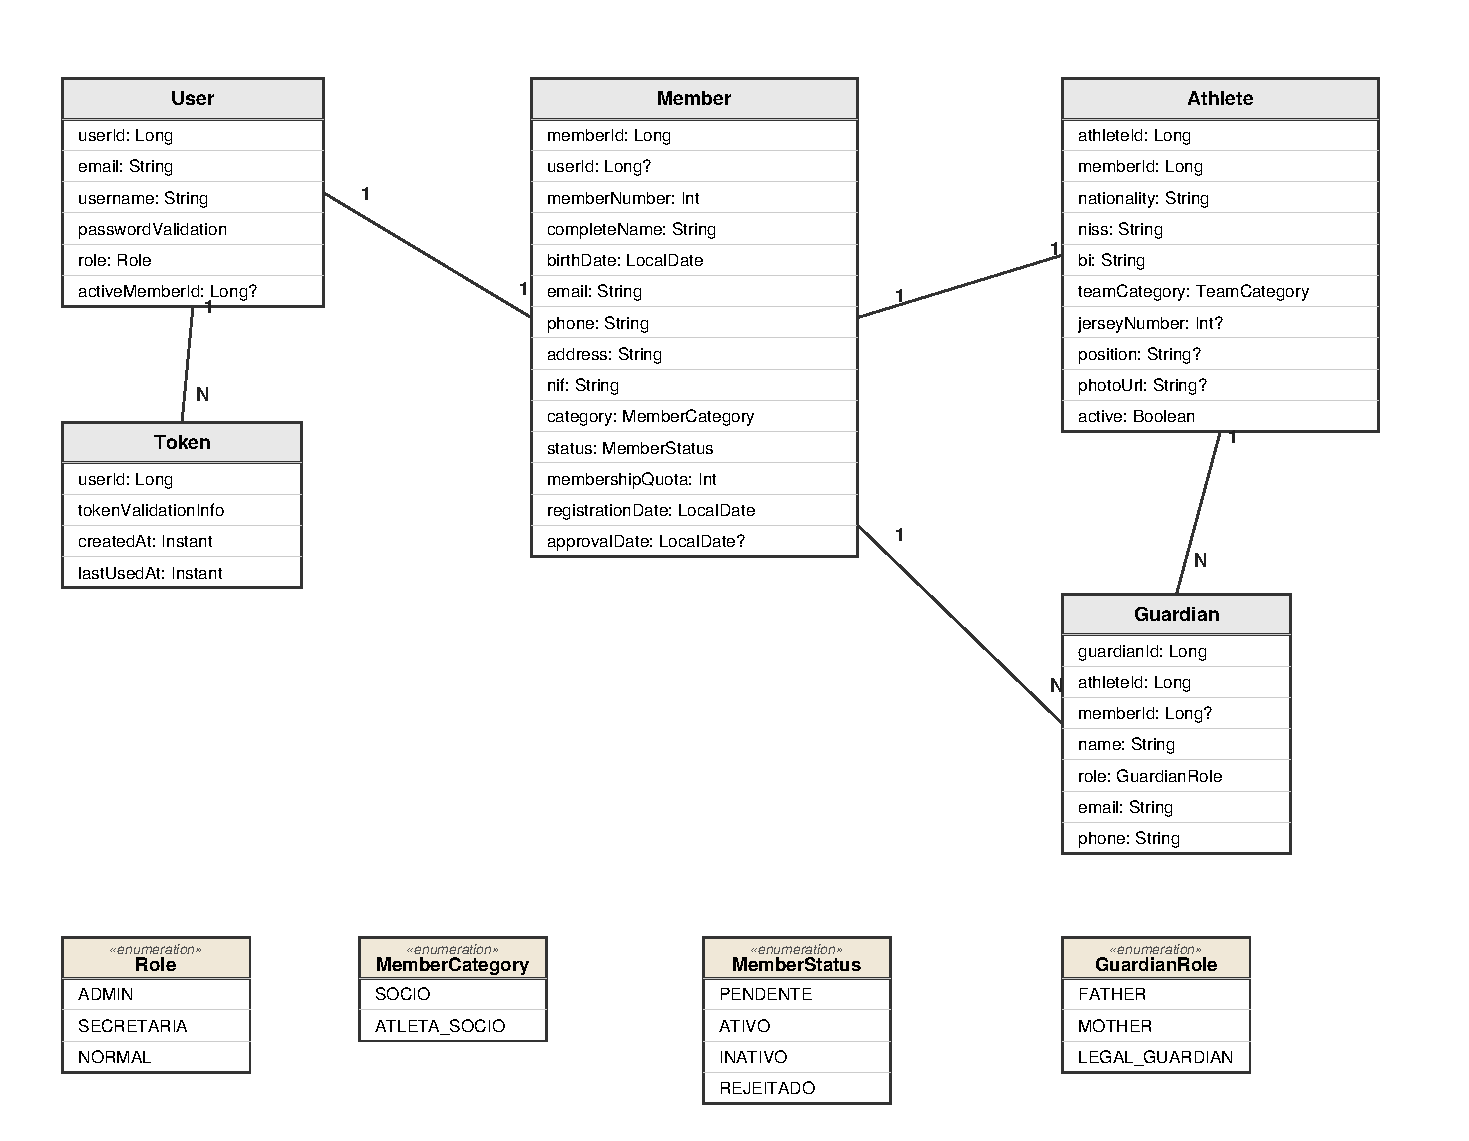
\includegraphics[width=\textwidth]{./figures/er-nucleo.pdf}
    \caption{Modelo de dados -- utilizadores, sócios e atletas}
    \label{fig:er-nucleo}
\end{figure}

\begin{figure}[H]
    \centering
    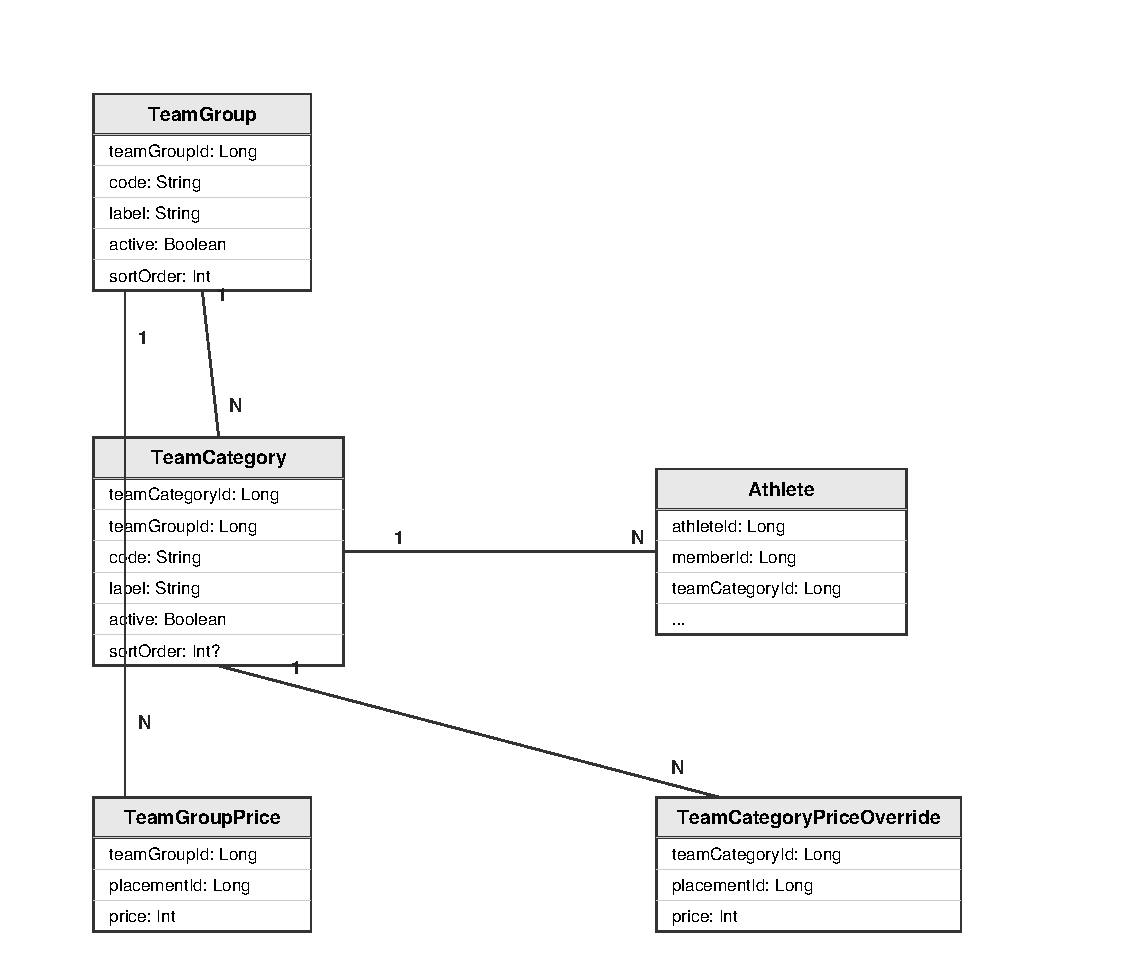
\includegraphics[width=0.75\textwidth]{./figures/er-equipas.pdf}
    \caption{Modelo de dados -- equipas e tabelas de preços}
    \label{fig:er-equipas}
\end{figure}

\begin{figure}[H]
    \centering
    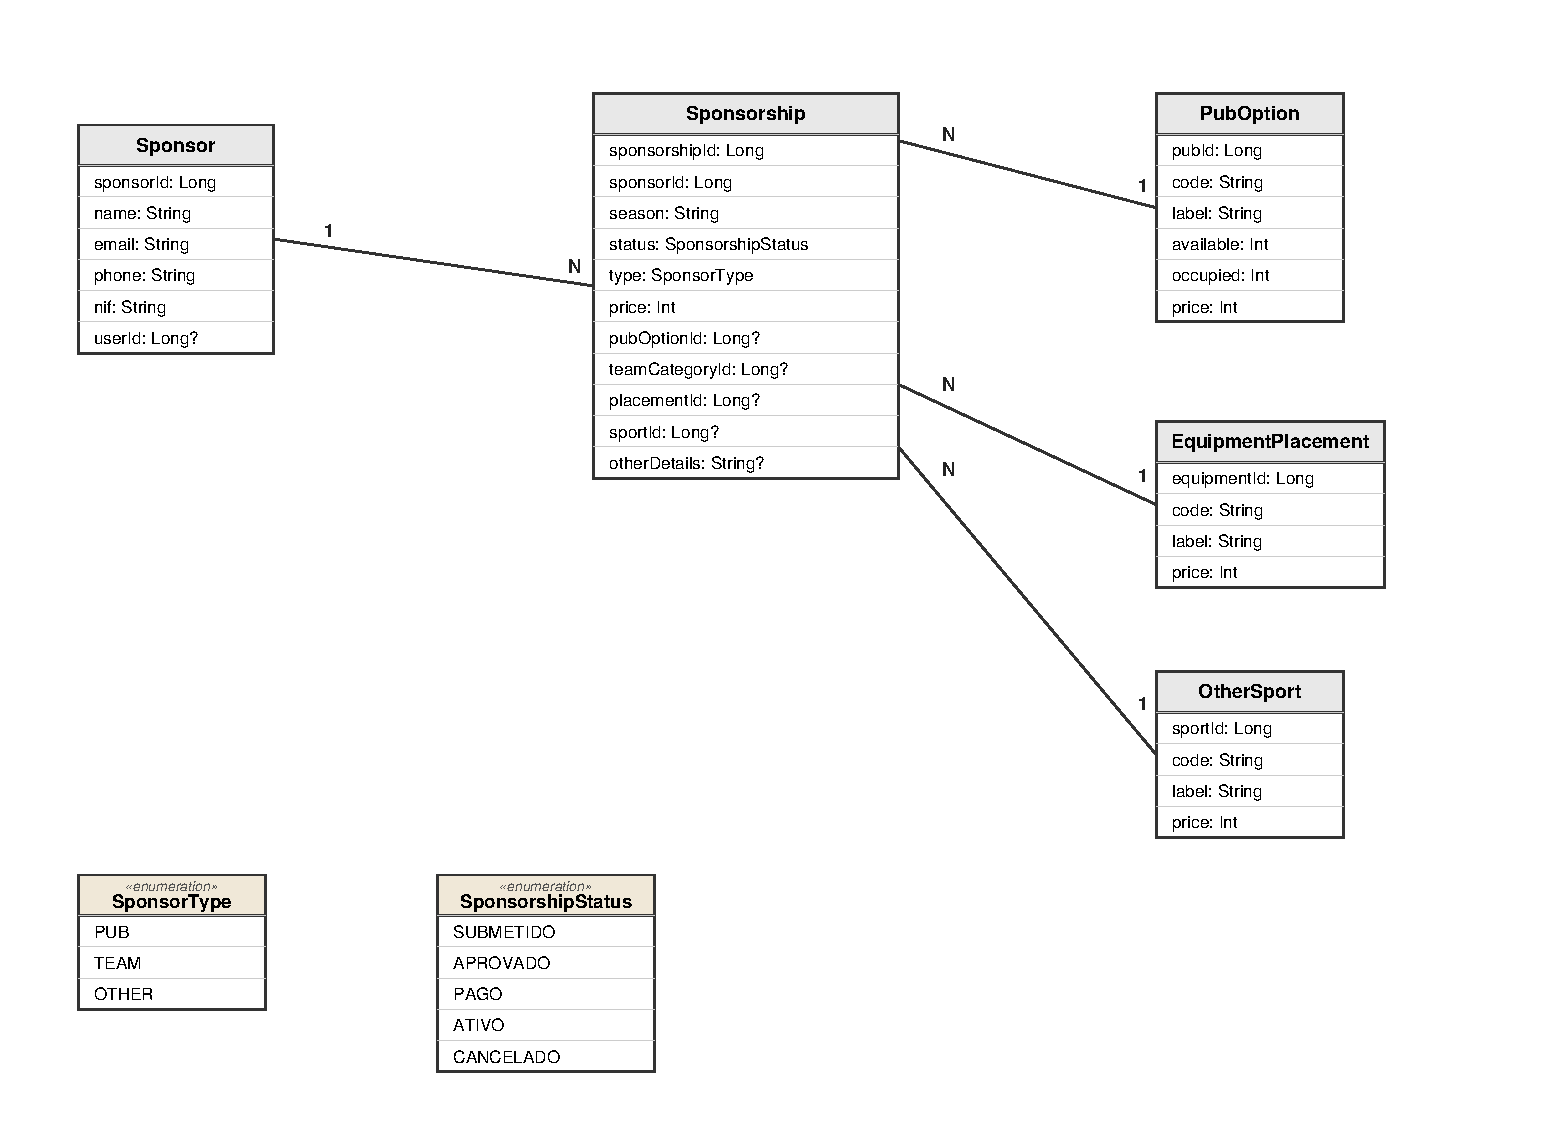
\includegraphics[width=\textwidth]{./figures/er-patrocinios.pdf}
    \caption{Modelo de dados -- patrocínios}
    \label{fig:er-patrocinios}
\end{figure}

\begin{figure}[H]
    \centering
    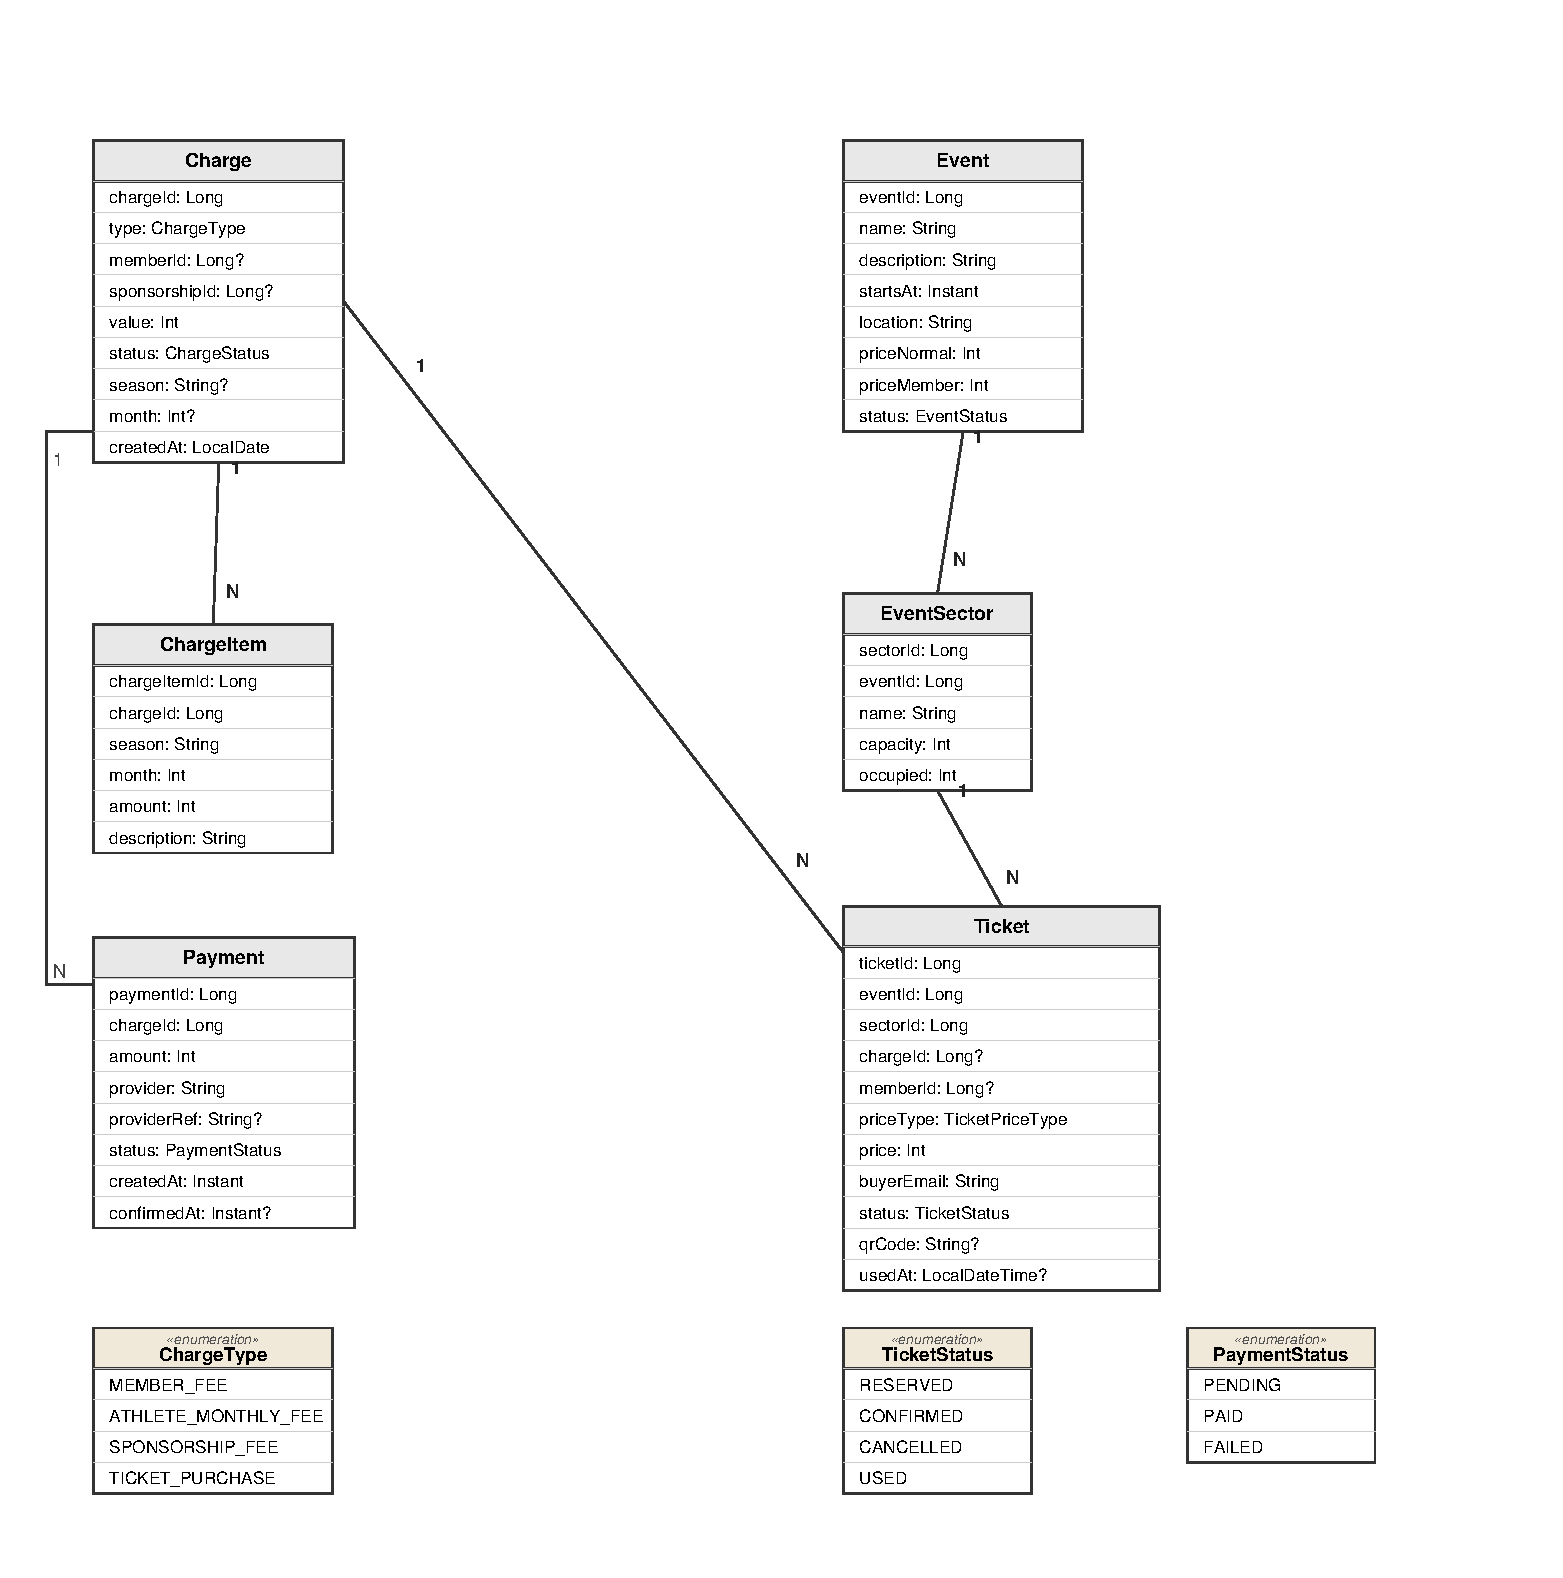
\includegraphics[width=0.85\textwidth]{./figures/er-financas-eventos.pdf}
    \caption{Modelo de dados -- cobranças, pagamentos e eventos}
    \label{fig:er-financas-eventos}
\end{figure}

\subsection{Repositório de Ficheiros}

O repositório de ficheiros é responsável pelo armazenamento de recursos 
binários associados às entidades da aplicação, nomeadamente fotografias de 
perfil, fotografias de sócios e atletas, e documentos como o cartão de cidadão 
ou o exame médico dos atletas.

Importa distinguir dois tipos de informação. Os \textit{metadados} de cada 
ficheiro -- como o nome original, o tipo de conteúdo, o tamanho e a chave de 
armazenamento -- são guardados na base de dados relacional, na entidade 
\texttt{StoredFile}. Já o conteúdo binário dos ficheiros não é guardado na base 
de dados, sendo delegado a um serviço de armazenamento externo, descrito em 
detalhe na Secção~\ref{sec:integracoes}.

Cada ficheiro é identificado por uma chave de armazenamento construída de forma 
hierárquica, que combina o tipo e o identificador da entidade proprietária, o 
tipo de ficheiro e um identificador único. É ainda aplicada uma política de um 
único ficheiro ativo por entidade e tipo, o que significa que o carregamento de 
um novo ficheiro substitui o anterior do mesmo tipo. O carregamento de 
ficheiros está sujeito a validações de tipo e tamanho, distintas consoante se 
trate de imagens ou de documentos.


\section{Serviços}

A camada de serviços é responsável pela lógica de negócio da aplicação. É nela 
que se realiza o processamento dos dados, a aplicação de regras e a 
orquestração das chamadas aos repositórios e aos serviços externos. Cada 
serviço é anotado com \texttt{@Named} e recebe as suas dependências por 
injeção no construtor, e recorre ao \texttt{TransactionManager} para que as 
operações que envolvem múltiplos repositórios sejam executadas no contexto de 
uma única transação.

Todos os serviços seguem uma abordagem de retorno funcional baseada no tipo 
genérico \texttt{Either<L, R>}, que encapsula o sucesso (\texttt{Right}) ou a 
falha (\texttt{Left}) de uma operação. Cada domínio define o seu próprio 
conjunto de erros, o que torna o tratamento de falhas explícito e evita o 
recurso a exceções não controladas. As operações de listagem seguem ainda um 
padrão uniforme de paginação, através das abstrações \texttt{Page} e 
\texttt{PageRequest}.

Existem vários serviços, cada um associado a uma área funcional da aplicação:

\begin{itemize}
    \item \texttt{UserService}: gere os utilizadores e as respetivas sessões, 
    incluindo a criação de utilizadores, a autenticação e a gestão de 
    \textit{tokens};
    \item \texttt{MemberService}: gere o ciclo de vida dos sócios, incluindo a 
    criação, aprovação, rejeição, ativação e desativação, bem como a alteração 
    de dados e de categoria;
    \item \texttt{AthleteService}: gere a inscrição e o ciclo de vida dos 
    atletas. A inscrição de um atleta cria, numa única transação, o sócio 
    associado, o atleta e os respetivos encarregados de educação;
    \item \texttt{EventService}: gere os jogos e a respetiva bilhética, 
    incluindo a criação de eventos e setores e o início do processo de compra 
    de bilhetes;
    \item \texttt{PaymentService}: coordena os pagamentos, as quotas e a 
    emissão de recibos, e integra-se com o serviço de pagamentos externo;
    \item \texttt{SponsorService} e \texttt{SponsorshipService}: gerem, 
    respetivamente, os patrocinadores e os contratos de patrocínio;
    \item \texttt{SponsorshipCatalogService} e \texttt{TeamService}: gerem os 
    catálogos de opções de patrocínio e a organização das equipas e tabelas de 
    preços;
    \item \texttt{AdminOverviewService}: agrega estatísticas para o painel de 
    administração;
    \item \texttt{FileService}: gere o carregamento, a consulta e a remoção de 
    ficheiros, aplicando validações de tipo e tamanho e verificando as 
    permissões de acesso;
    \item \texttt{EmailService}: compõe e envia mensagens de correio 
    eletrónico.
\end{itemize}

A maioria destes serviços segue um modelo simples e consistente: recebem os 
dados, validam as regras de negócio, interagem com os repositórios 
correspondentes e retornam o resultado da operação. Por esse motivo, não são 
detalhados individualmente. O \texttt{PaymentService}, pela sua complexidade e 
pela integração com serviços externos, é descrito em detalhe na 
Secção~\ref{sec:integracoes}.

\section{Controladores}

No contexto da \textit{framework} Spring, um controlador (ou 
\textit{controller}) é o componente responsável por receber e tratar os 
pedidos HTTP efetuados pelos clientes. Estes pedidos são originados a partir da 
aplicação \textit{frontend}, que comunica com o \textit{backend} através de uma 
Web API REST. A função principal de um controlador é interpretar os dados 
recebidos, invocar os serviços adequados e devolver uma resposta apropriada, 
normalmente em formato JSON. Para este efeito, foi utilizada a anotação 
\texttt{@RestController}, apropriada para aplicações que não retornam páginas 
HTML, mas sim dados em formato JSON.

Existem vários controladores na aplicação, cada um responsável por um conjunto 
específico de \textit{endpoints}. Os principais são:

\begin{itemize}
    \item \texttt{UserController}: criação de utilizadores, autenticação 
    (\textit{login} e \textit{logout}) e obtenção da informação do utilizador 
    autenticado;
    \item \texttt{MemberController}: criação, consulta, atualização e gestão do 
    ciclo de vida dos sócios;
    \item \texttt{AthleteController}: inscrição de atletas, consulta pública 
    por escalão e gestão administrativa dos atletas;
    \item \texttt{EventController}: criação e gestão de jogos, consulta de 
    eventos disponíveis e início do processo de compra de bilhetes;
    \item \texttt{PaymentController}: criação de sessões de pagamento, gestão 
    de quotas, emissão de recibos e receção de notificações do serviço de 
    pagamentos;
    \item \texttt{SponsorController} e \texttt{SponsorshipController}: gestão de 
    patrocinadores e de contratos de patrocínio;
    \item \texttt{SponsorshipCatalogController} e \texttt{TeamController}: 
    gestão dos catálogos de patrocínio e da organização das equipas;
    \item \texttt{AdminController}: obtenção de estatísticas para o painel de 
    administração;
    \item \texttt{FileController}: carregamento, consulta e remoção de 
    ficheiros.
\end{itemize}

Importa notar que os controladores que requerem autenticação recebem um objeto 
com a informação do utilizador autenticado, injetado automaticamente pela 
aplicação, como detalhado na Secção~\ref{sec:autenticacao}.

Além da separação clara de responsabilidades, os controladores seguem um 
estilo coeso de tratamento de erros. A aplicação adota o padrão 
\textit{Problem Details for HTTP APIs} (RFC 7807), que devolve 
respostas de erro com uma estrutura unificada em formato JSON, com campos como 
\texttt{type}, \texttt{title}, \texttt{status} e \texttt{detail}, que permitem 
compreender de forma padronizada a natureza do erro ocorrido. A conversão dos 
erros internos de cada domínio para este formato é feita de forma centralizada.

\section{Autenticação e Autorização}
\label{sec:autenticacao}

A autenticação dos utilizadores assenta num mecanismo de \textit{tokens} 
opacos, gerados pela aplicação e persistidos na base de dados. Ao contrário de 
uma palavra-passe, o \textit{token} não transporta qualquer informação 
legível: é apenas uma credencial aleatória que o servidor sabe associar a um 
utilizador. As palavras-passe dos utilizadores nunca são armazenadas em texto 
simples, sendo guardada apenas a sua representação cifrada através do algoritmo 
\textit{BCrypt}.

O processo de autenticação segue os seguintes passos:

\begin{enumerate}
    \item O utilizador submete as suas credenciais (nome de utilizador ou 
    \textit{email}, e palavra-passe);
    \item O servidor procura o utilizador correspondente e valida a 
    palavra-passe submetida contra a representação cifrada armazenada;
    \item Em caso de sucesso, é gerado um \textit{token} aleatório, do qual é 
    guardada na base de dados apenas uma representação cifrada 
    (\textit{hash} SHA-256);
    \item O \textit{token} é devolvido ao cliente, tanto no corpo da resposta 
    como num \textit{cookie} seguro (\texttt{HttpOnly}), utilizado nos pedidos 
    seguintes.
\end{enumerate}

Cada \textit{token} tem associado um tempo de validade absoluto e um tempo de 
validade por inatividade, sendo ainda limitado o número máximo de 
\textit{tokens} ativos por utilizador. A validação dos pedidos autenticados é 
feita de forma centralizada por um \textit{interceptor}, que é executado antes 
dos controladores. Este componente extrai o \textit{token} do cabeçalho de 
autorização (ou, em alternativa, do \textit{cookie}), valida-o e, em caso de 
sucesso, disponibiliza a informação do utilizador autenticado ao controlador. 
Caso a validação falhe, o pedido é rejeitado com o código de estado HTTP 401.

No que diz respeito à autorização, a aplicação define três papéis: 
\texttt{ADMIN}, \texttt{SECRETARIA} e \texttt{NORMAL}. Os papéis 
\texttt{ADMIN} e \texttt{SECRETARIA} partilham o acesso às funcionalidades de 
gestão (\textit{backoffice}), enquanto o papel \texttt{NORMAL} corresponde ao 
utilizador comum. A verificação de permissões é feita ao nível dos serviços e 
dos controladores. Para além da verificação por papel, existe também uma 
verificação de propriedade do recurso, que garante, por exemplo, que um 
utilizador só pode pagar ou consultar dados que lhe dizem respeito.

\section{Integrações Externas}
\label{sec:integracoes}

O \textit{backend} integra-se com vários serviços externos para suportar 
funcionalidades que não fazem parte do seu domínio central. Esta secção 
descreve essas integrações.

\subsection{Pagamentos com Stripe}

O processamento de pagamentos é feito através da plataforma Stripe~\cite{stripe}, 
que trata de toda a interação com os meios de pagamento, sem que os dados 
bancários dos utilizadores passem pelo servidor da aplicação. A integração é 
coordenada pelo \texttt{PaymentService} e suporta diferentes tipos de cobrança: 
quotas de sócio, mensalidades de atleta, patrocínios e compra de bilhetes.

O fluxo de pagamento decorre da seguinte forma:

\begin{enumerate}
    \item O cliente inicia o pagamento através do \textit{endpoint} 
    correspondente;
    \item O \textit{backend} cria a cobrança e os respetivos itens, regista um 
    pagamento no estado pendente e cria uma sessão de pagamento na Stripe, 
    devolvendo ao cliente o endereço para onde deve ser redirecionado;
    \item Após a conclusão do pagamento, a Stripe notifica o \textit{backend} 
    através de um \textit{webhook};
    \item O \textit{backend} valida a autenticidade da notificação e, em caso 
    de sucesso, confirma o pagamento e a cobrança, atualiza o estado das 
    entidades associadas (por exemplo, confirma os bilhetes e gera os 
    respetivos códigos QR) e envia uma mensagem de confirmação ao utilizador. 
    Em caso de falha, o pagamento é marcado como falhado e os recursos 
    reservados são libertados.
\end{enumerate}

A validação da autenticidade das notificações é feita através da verificação de 
uma assinatura, o que impede que pedidos forjados sejam aceites como 
pagamentos válidos.

\subsection{Envio de Correio Eletrónico}

O envio de mensagens de correio eletrónico é suportado pelo módulo de 
\textit{email} do Spring, configurado para comunicar com um servidor SMTP 
externo. A composição das mensagens é da responsabilidade do 
\texttt{EmailService}, que gera conteúdo em HTML. A principal utilização atual 
é o envio da confirmação de compra de bilhetes, na qual os códigos QR são 
incluídos como imagens incorporadas na própria mensagem.

\subsection{Armazenamento de Ficheiros}

O conteúdo binário dos ficheiros não é guardado na base de dados, mas sim num serviço de armazenamento 
externo. A aplicação utiliza o serviço Cloudflare R2, acedido através de uma 
API compatível com o protocolo S3 da Amazon. O acesso ao armazenamento é 
abstraído por uma interface, o que permite, no futuro, substituir o serviço 
utilizado sem alterar a lógica da aplicação. Este serviço é utilizado para 
armazenar fotografias de perfil, fotografias de sócios e atletas, e documentos 
associados aos atletas.

\subsection{Geração de Códigos QR}

A geração dos códigos QR utilizados na bilhética é feita através da biblioteca 
ZXing~\cite{zxing}. A partir de um identificador único associado a cada 
bilhete, é gerada uma imagem que é posteriormente incluída na mensagem de 
confirmação de compra enviada ao utilizador.